\documentclass[11pt]{scrarticle}
% Essential packages
\usepackage{graphicx}         % For including graphics/images
\usepackage{xcolor}           % For color text and colored elements
\usepackage{hyperref}         % For clickable hyperlinks in PDF
\usepackage[T1]{fontenc}      % Use T1 font encoding (better handling of accented characters)
\usepackage{amsmath,          % American Mathematical Society math extensions
            amsfonts,         % Additional math fonts
            amssymb,          % Additional math symbols
            amsthm,           % Theorem environment support
            mathtools}        % Enhances amsmath with extra tools

\usepackage{csquotes}         % Context-sensitive quotation marks, required by biblatex
\usepackage[english]{babel}   % Language-specific typography and hyphenation (here: English)

% Captioning and subfigures
\usepackage{caption}          % Customizing captions
\usepackage{subcaption}       % Sub-figures and sub-tables

% Tables and tabular enhancements
\usepackage{longtable}        % Multi-page tables
\usepackage{array}            % Extends tabular environment
\usepackage{multirow}         % Table cells spanning multiple rows
\usepackage{wrapfig}          % Wrapping text around figures
\usepackage{colortbl}         % Color in tables
\usepackage{pdflscape}        % Landscape pages in PDF (auto-rotating)
\usepackage{tabu}             % Flexible tables (now outdated and deprecated)
\usepackage{threeparttable}   % Notes under tables
\usepackage{threeparttablex}  % Extended version of above with longtable support
\usepackage{makecell}         % Custom line breaks and formatting in table cells
\usepackage{siunitx}          % Proper typesetting of units and numbers
\usepackage{float}            % Improved float positioning (e.g., [H] specifier)
\usepackage{booktabs}         % Professional-quality tables (rules, spacing)

% Fonts and spacing
\usepackage{lmodern}          % Latin Modern font (scalable, better for PDF)
\usepackage{setspace}         % Control line spacing
\usepackage[bottom]{footmisc} % Place footnotes at bottom of page consistently

% Bibliography
\usepackage[style = apa]{biblatex} % APA citation style using biblatex
\addbibresource{../bibliography/bibliography.bib} % Bibliography file

% Layout
\usepackage[a4paper, vmargin=3.3cm, hmargin=3.3cm]{geometry} % Set page size and margins

% Prevent widows/orphans
\widowpenalty=10000 % Avoid single lines of paragraphs at the top/bottom of pages

% KOMA-Script settings
\addtokomafont{disposition}{\rmfamily} % Use roman font for section headings

% Custom title formatting
\makeatletter
\renewcommand{\maketitle}{
  \begin{center}
    {\usekomafont{title}{\LARGE\@title\par}}%
    \vskip 1em 
    {\usekomafont{subtitle}{\large\@subtitle\par}}%
    \vskip 1em   
    {\usekomafont{author}{\@author\par}}%
  \end{center}
}
\makeatother

% Hyperref customization
\hypersetup{
        unicode = false,                    % non-Latin characters in Acrobat’s bookmarks
        pdftoolbar = true,                  % show Acrobat’s toolbar?
        pdfmenubar = true,                  % show Acrobat’s menu?
        pdffitwindow = false,               % window fit to page when opened
        pdfstartview = {FitH},              % fits the width of the page to the window
        pdftitle = {},                      % title
        pdfauthor = {},     % author
        pdfsubject = {Subject},             % subject of the document
        pdfcreator = {},    % creator of the document
        pdfproducer = {},                   % producer of the document
        pdfkeywords = {},                   % list of keywords
        pdfnewwindow = true,                % links in new PDF window
        colorlinks = true,                  % false: boxed links; true: colored links
        linkcolor = teal,                   % color of internal links (change box color with linkbordercolor)
        citecolor = teal,                   % color of links to bibliography
        filecolor = cyan,                   % color of file links
        urlcolor = red                      % color of external links
    }   

% Spacing configuration
\setstretch{1.25}                      % Single line spacing
\setlength{\parindent}{15pt}       % Paragraph indentation
\setlength{\parskip}{2.5pt}          % Spacing between paragraphs
\setlength{\skip\footins}{15pt}    % Spacing before footnotes

% Image settings
\setkeys{Gin}{keepaspectratio}     % Maintain image proportions when scaling

% Title
\title{Farm-to-factory? Peasant Unrest and Surveillance in Late Imperial Russia}
\subtitle{Political Economy of Democracy}
\author{Stepan Polikanov}

% Document
\begin{document}

\maketitle

\section{Introduction}

Why did democratization in the Russian Empire fail to take root, despite the appearance of representative institutions such as the State Duma in the early 20th century? This paper approaches that question by studying not democratization’s emergence, but its absence. Focusing on the structure of peasant unrest and the Tsarist regime’s selective repression, I argue that institutional responses to rural mobilization reveal the barriers to political inclusion embedded in the post-emancipation social order.

Theoretically, the analysis begins with the legacy of serfdom: a deeply entrenched system that sustained elite dominance through legal and territorial control over the peasantry. Even after formal abolition in 1861, serfdom’s shadow persisted in the communal landholding system (mir), land inequality, and restricted peasant agency. These features created not only economic hardship but also political frustration. Peasant unrest, particularly in the decades following emancipation, reflected this discontent—not as isolated violence, but as a form of collective negotiation under conditions of unfulfilled reform.

However, the Russian autocracy did not incorporate these bottom-up demands into a broadened political contract. Instead, it deployed repression selectively, often preemptively, in regions with high unrest and mobilization potential. The Tsarist regime's coercive institutions—primarily the military and the Okhrana\footnote{Tsarist political police} not just ideological revolutionaries but also those who embodied the rural question within urban political movements. This is particularly evident in the "farm-to-factory" dynamic: former peasants migrating seasonally into cities brought with them unresolved agrarian grievances, which fused with labor radicalism and increasingly drew the state’s surveillance.

In this sense, the Russian case is a negative instance in the broader political economy of democratization. Where democratization elsewhere often emerged from elite bargains in response to credible threats from below, the Empire’s strategy was not co-optation but insulation. As recent research of \cite{dower_collective_2017} and \cite{finkel_does_2015}, even moments of apparent institutional opening were structured to neutralize peasant influence through curial voting and overrepresentation of conservative estates. The findings presented here suggest that repression filled the gap where incorporation proved politically intolerable.

By linking pre-1905 peasant unrest to the spatial intensity of Okhrana surveillance, this paper traces how long-run social structures shaped short-run political strategies. It contributes to the political economy of authoritarianism by showing how historical grievances, migration patterns, and institutional design jointly conditioned the limits of imperial reform.

First, it contributes to the political economy of authoritarianism by demonstrating how autocratic regimes respond to localized protest not with uniform coercion but with selective, spatially differentiated repression. In this sense, it aligns with work on strategic state violence and surveillance \parencite{greitens_dictators_2016,dimitrov_why_2013}, while offering new empirical evidence from a pre-Soviet context.

Second, it adds to the literature on the legacies of coercive institutions, particularly the afterlives of serfdom, by showing how historical systems of labor control shaped both the capacity for and the perception of threat by the state decades later. This builds on research in economic history and development (e.g., \cite{buggle_slow_2021,markevich_economic_2018}) and brings it into conversation with political mobilization and repression.

Third, it engages with debates in historical sociology and contentious politics, showing how rural collective action shaped elite institutional responses even in the absence of programmatic demands. The paper thus speaks to theories of protest and state formation \parencite{tilly_mobilization_1978,slater_ordering_2010}, emphasizing grievance-based, non-institutionalized mobilization as a driver of autocratic institutional behavior.

Fourth, it makes a novel contribution to the political economy of democratization by presenting the Russian case as a negative trajectory—a case where elite fears of redistribution and loss of control resulted not in negotiated inclusion but in intensified repression. In doing so, it complements existing theories of elite-initiated democratization \parencite{acemoglu_economic_2005,gandhi_authoritarian_2007}, while highlighting the institutional fragility of concession-based reforms in estate-based polities.
 
\section{Theoretical framework}

\subsection{Legacies of serfdom}

For much of the Russian Empire’s history, serfdom formed the backbone of its agrarian economy, social hierarchy, and political order. By the mid-19th century, roughly one-third of the empire’s population — and over 50\% of the peasantry in central regions — were bound by forms of personal and economic dependence that left them legally subordinate and territorially immobile. Serfs were tethered to noble landlords through a system of customary obligations and judicial inequality, performing labor services or paying rents while lacking the right to freely move, contract, or petition the state independently \parencite{dennison_institutional_2011,gerschenkron_economic_1979}. Unlike chattel slavery, serfdom in Russia entailed communal obligations and paternalistic oversight rather than commodified ownership, but its effects on social stratification were no less severe.

The institution was not merely economic — it was deeply political. Serfdom entrenched elite control over both land and legal authority, making the local nobility indispensable to imperial administration. In return for their loyalty, landlords were granted wide discretion over judicial and fiscal matters on their estates. This created a dual state: a formal imperial bureaucracy and a shadow structure of private rule. As \cite{boucoyannis_kings_2021} and \cite{dower_collective_2017} suggest, this arrangement inhibited the development of representative institutions and discouraged state-building from below. Where other European polities saw gradual incorporation of peasant interests into local governance or national assemblies, the Russian state relied on a coercive agrarian order that marginalized peasant political agency and blocked pathways to participation.

Though serfdom was formally abolished in 1861, its institutional and social structures persisted deep into the late 19th century, shaping the material conditions and political identities of the Russian peasantry. Emancipation created a class of legally free but economically constrained rural producers. The 1861 reform granted land not as private property, but as \textit{nadel} allotments distributed through the communal landholding institution (\textit{mir}), reinforcing a system that preserved hierarchical dependence and impeded upward mobility. As numerous scholars have shown, this arrangement failed to meaningfully redistribute productive land, leaving former serfs with small, fragmented plots and subject to redemption payments to their former landlords \parencite{markevich_economic_2018,gerschenkron_economic_1979,buggle_slow_2021}.

These post-reform structures institutionalized deprivation. While communal governance offered internal cohesion, it also operated under state surveillance and favored vertical compliance over horizontal mobilization \parencite{dennison_living_2012}. The \textit{mir} system limited market participation and formalized the peasant’s subordination within the local estate hierarchy, often mediated by noble-dominated zemstvo councils. As \cite{popov_factors_2023} and \cite{finkel_does_2015} show, the mismatch between legal emancipation and continued material inequality created a volatile political terrain. Peasants were legally recognized as autonomous persons but were institutionally contained through systems that precluded effective control over land, credit, or legal recourse.

While these structural inequalities created fertile ground for discontent, their translation into state repression was not automatic. As the empirical analysis will show, inequality alone did not predict coercion—suggesting that it was the politicization, not just the presence, of inequality that mattered.

\subsection{Peasant unrest}

It was in this institutional context that the Russian peasantry developed distinct repertoires of collective action. Peasant unrest was not merely episodic violence or irrational revolt—it was a form of reactive and adaptive political behavior. Drawing on long-standing communal norms of mutual aid and grievance redress, peasants mobilized to contest the unfulfilled promises of reform. As \cite{finkel_does_2015} argue, the very structure of the post-emancipation settlement encouraged protest: it clarified legal expectations without delivering meaningful autonomy or land security.

Between the 1850s and 1870s, Russia experienced waves of rural disturbances that varied in scale and form. Some incidents focused narrowly on land seizures or tax refusals; others evolved into protracted confrontations with local officials, landlords, and police. The peasant movement was spatially uneven but politically coherent. Regions with high serf populations prior to 1861—and especially those with persistent land inequality—were more likely to experience violent unrest \cite{kofanov_land_2020}. \cite{dower_collective_2017} and \cite{popov_factors_2023} show that unrest was particularly acute in areas where the communal landholding system failed to mitigate inequality or was manipulated by local elites.

This form of protest—while lacking formal leadership or consistent ideological framing—was rooted in shared experiences of economic injustice and legal disappointment. Its intensity stemmed not from revolutionary doctrine but from the practical impossibility of making a living under post-reform constraints. In this sense, peasant unrest in late imperial Russia was a form of institutional negotiation from below,” in which demands for access to land and autonomy were staged against a background of formal emancipation and persistent subjugation.

These uprisings did not go unnoticed by the state. Not only did they trigger alarm about agrarian stability, they were also seen as precursors to more organized revolutionary activity. Indeed, unrest was a key channel through which rural discontent entered the political consciousness of urban radicals, leftist parties, and the state’s coercive apparatus. It is precisely in this context that the state’s eventual turn to targeted repression — and the institutional development of both military suppression and Okhrana surveillance — must be understood.

\subsection{State responses to bottom-up threats}

Across autocratic and transitional regimes, the state’s response to grassroots mobilization is shaped not solely by the presence of unrest, but by the perceived threat such mobilization poses to elite control. A substantial body of literature argues that regimes respond to bottom-up pressure with a strategic mix of repression, concession, and co-optation \parencite{tilly_mobilization_1978,davenport_state_2007,gandhi_authoritarian_2007}. Whether a regime chooses to incorporate dissenters into institutions or exclude and punish them depends on how threatening it judges their demands to be, and on the feasibility of containing them without altering elite privileges.

In autocracies in particular, where elites are often wary of institutionalizing mass participation, repression emerges as a default tool for neutralizing threats from below. Unlike democracies, where incorporation may increase regime legitimacy or stability, autocracies have fewer incentives to broaden participation when doing so threatens elite interests. The logic is captured by \cite{acemoglu_economic_2005}: elites concede power only when repression is either too costly or ineffective. Otherwise, the status quo is maintained by force or threat thereof.

Repression, then, is not merely a reaction to disorder — it is a preemptive political choice \parencite{dimitrov_why_2013}. As \cite{greitens_dictators_2016} and \cite{slater_ordering_2010} both emphasize, autocratic leaders invest in coercive institutions and deploy them selectively, especially in regions where collective action capacity is already high. This strategic deployment ensures that repression is cost-efficient: resources are concentrated where unrest is most threatening to regime continuity, typically areas with a record of protest or existing mobilization structures. Indeed, following \cite{greitens_dictators_2016} typology, regimes facing mass protest invest in internal security institutions such as secret police and surveillance, while those concerned about elite defection focus on coup-proofing strategies. 

In the Russian Empire, mass unrest suppression was a dedicated domain of the military throughout the XIX century. By the early 20th century, the Russian autocracy had already experienced significant rural unrest, most notably during and after the 1861 emancipation. The peasantry, though disenfranchised and institutionally marginalized, remained a large, often discontented segment of society. It was also increasingly politicized — not in a partisan sense, but through exposure to land struggles, redemption payments, commune conflicts, and the experience of collective protest. The 1905 revolution underscored the growing threat: peasant uprisings were widespread and increasingly coordinated. From the perspective of the Tsarist regime, repression was a rational and targeted response to this rising mobilization.

On the other hand, the secret police, \textit{Okhrana}, formed in 1881, was a product of a rapidly developing political arena that offered a left-wing ideological voice to the disenchanted peasanty and workers. Okhrana institutions were charged with defending the state from both organized revolutionary threats and, increasingly, from the diffuse politicization of society itself \parencite{daly_autocracy_1998}. To some extent, one can think of the military and Okhrana as complementary and specialized responses to different kind of threats. Whilst general peasant dicontent was chiefly handled by military suppression, when it started penetrating previously sequestered political arenas, finer and more precise tools became needed. Indeed, as \cite{daly_autocracy_1998} shows, the boundaries blurred. Peasant unions and agrarian activists became of central concern to the security police by 1905, as the state realized that the real danger lay not just in spontaneous disorder, but in the amalgamation of grievances into cohesive political demands.

What distinguished the Okhrana from the army was not only its bureaucratic specialization but its informational logic. Rather than suppressing mass protest through sheer force, it aimed to prevent its coordination through intelligence. Officers developed complex schematic diagrams tracking personal and professional relationships among suspects. By 1901, the Special Section maintained a library of over 5,000 banned publications and constructed social network charts of revolutionary groups with up to 200 nodes \parencite{daly_autocracy_1998}. These efforts represent what \cite{dimitrov_why_2013} terms ``preemptive authoritarianism'' — the use of surveillance to detect and neutralize threats before they materialize as mass mobilization.

Thus, I approach repression not as a sign of state weakness, but as an instrument of elite rule maintenance in the face of bottom-up demands for redistribution, access, or reform. The state’s behavior in the aftermath of the 1905 revolution — the surveillance of rural activists, the manipulation of curial representation, the selective use of police and military power — fits squarely into this broader pattern of selective coercion in the service of institutional insulation. More importantly, in the Russian Empire, concessions made to political calls of peasantry were always partial - the 1861 abolition of serfdom, zemstvos established shortly after, the 1905 State Duma were all angled at preserving the conservative order rather than actual arenas for agonistic politics. Inability of the state to institute effective cooption that was unnerving to landowner stakeholders meant that repression was required for regime survival.

In this framework, unrest functions less as a direct cause of repression and more as a signal—a spatially legible proxy for regions where collective action capacity exists or might emerge. It is not the violence per se that attracts coercion, but the potential for coordination and ideological activation that unrest reveals to the regime.

\subsection{Farm-to-Factory? Labour migration and urban lives of peasants}

If much of the previous section has dealt with rural unrest in its own terms, there remains the question of how, if at all, these structurally embedded grievances came to matter in the urban, ideologically coded space that defined late imperial repression. Urban repression, particularly at the hands of the Okhrana, is typically studied in terms of its ideological targets: revolutionaries, radicals, syndicalists, underground cells. Yet the social origins of these ideological actors, as well as the conditions under which ideology became fused with class-based grievance, remain central to understanding why certain populations attracted disproportionate attention from the state.

Urban population of Russian cities doubled from 1867 to 1897, with \cite{gatrell_tsarist_1986} attributing most of the growth to migration from the countryside. The pattern was strongly regional: in 1869, and again in 1910, most of those moving into cities came either from the province the city was located in or from its immediate neighbors \parencite{gatrell_tsarist_1986}. The overwhelming majority of these migrants were of peasant estate background \parencite{fauser_engines_2021}. This alone suffices to establish the demographic shift — that peasant-origin individuals were entering, and eventually reshaping, the social composition of the cities.

Whether these individuals retained enough of the rural grievance repertoire to influence urban political dynamics is a separate, and more theoretically interesting, question. Here the nature of migration becomes crucial. Due to the seasonality of agricultural work and the structural obligations of redemption payments on communal land allotments (\textit{nadels}), the practice of \textit{otkhodnichestvo} — seasonal wage migration — became widespread. Peasants traveled to urban centers in non-agricultural months to earn cash wages, typically remitting them to their home villages in order to meet financial obligations or support kin \parencite{fauser_engines_2021}. On the other hand, they experienced all the modernity and cultural life found in the cities. They were, as Johnson puts it, ``living in the city without being fully of the city'' \parencite{johnson_paradigms_2010}. This mode of presence preserved not only social ties to the rural commune but also the ideological framing of land as a fundamental injustice. 

Industrialization and the expansion of the rail network further deepened this rural-urban entanglement. Migrants could travel further, more frequently, and with less permanent dislocation. By the early 20\textsuperscript{th} century, land inequality had become a central theme in revolutionary rhetoric, despite being a question formally tied to the village. This is not coincidental. As I argue, the material substance of peasant grievance — unmet expectations of emancipation, coercive communal tenure, and elite capture of local governance — found its ideological voice not in the commune, but in the factory floor and the party cell.

This opens up a reinterpretation of the logic of repression. While the Okhrana focused operationally on the urban underground, its targets often embodied the rural question — by origin, by rhetoric, or by imagined constituency. The peasant estate, in this reading, was not just a legal status; it was a heuristic of political volatility. The state responded accordingly: repression followed not only where ideology was thickest, but where it appeared most contaminated by unresolved class antagonism from the countryside. Though this rural-urban transmission is difficult to observe directly in the available data, the pattern of Okhrana repression aligning with urban centers that absorbed high peasant migration offers circumstantial support. This mechanism remains a theoretically inferred link rather than a directly measured causal pathway.

\section{Data}

This paper draws primarily on archival data on political policing compiled by \cite{grigoriadis_data_2024}, documenting activities of the Tsarist Okhrana. The dataset covers over 13,000 cases between the 1880s and 1917, including geographic location, year, and the data source label (e.g., \textit{accused}, \textit{revolutionaries}). Despite substantial missingness in individual-level demographic variables (e.g., rank, education, ethnicity), the geographic metadata is robust. I focus on counts of Okhrana cases by province, using a variety of sources from other studies.

I match this outcome data with structural predictors from the broader imperial context. These include:

\begin{itemize}
    \item \textbf{Peasant unrest}: number of collective disturbances recorded between 1851 and 1871 \cite{finkel_does_2015}.
    \item \textbf{Land inequality}: Gini coefficient of landholding calculated from 1905 land records (\cite{lindert_russian_2014} and see the Appendix for the calculation).
    \item \textbf{Serf legacy}: share of population held in serfdom in 1858 \cite{markevich_economic_2018}.
    \item \textbf{Peasant land deprivation}: share of land held by peasants \parencite{lindert_russian_2014}.
    \item \textbf{Urban and industrial indicators}: urbanization rate and share of manufacturing in the economy, from 1897 and 1904 records \parencite{lindert_russian_2014}.
\end{itemize}

\section{Research Design}

\subsection{Descriptive Patterns}

I begin by visualizing the geographic distribution of Okhrana activity. I use geocoded provinces from the 1897 census for maps, prepared by \cite{kessler_electronic_2020}. Mapping case frequency by province highlights significant heterogeneity, with certain regions such as the Pale of Settlement, central Ukraine, and urbanized industrial centers showing elevated surveillance and repression. 

\begin{figure}
  \centering
  \caption{Okhrana cases by province (Grigoriadis, 2025)}
  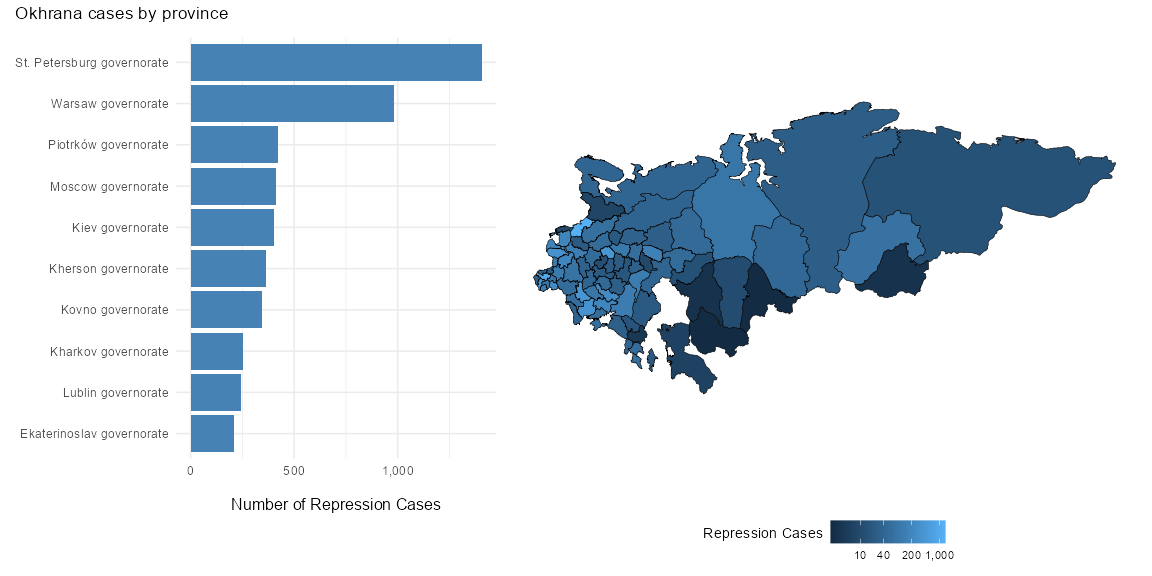
\includegraphics[width = \textwidth]{okhrana_by_province.png}
\end{figure}

\subsection{Empirical Models}

The main analytical task is to identify predictors of Okhrana surveillance intensity at the province level. The dependent variable is the logged number of Okhrana cases per province, as captured in the archival dataset. We estimate a sequence of nested linear and count models:

\begin{align*}
    \text{Model 1:} \quad & y_i = \beta_0 + \beta_1 \cdot \log(\text{Unrest}_i + 1) + \epsilon_i \\
    \text{Model 2:} \quad & y_i = \beta_0 + \beta_1 \cdot \log(\text{Unrest}_i + 1) + \beta_2 \cdot \text{LandIneq}_i + \epsilon_i \\
    \text{Model 3:} \quad & y_i = \beta_0 + \beta_1 \cdot \log(\text{Unrest}_i + 1) + \beta_2 \cdot \text{LandIneq}_i + \beta_3 \cdot \text{Serfs}_i + \beta_4 \cdot \text{PeasantLand}_i + \epsilon_i \\
    \text{Model 4:} \quad & \text{Model 3} + \beta_5 \cdot \text{Urban}_i + \beta_6 \cdot \text{Manufacturing}_i + \epsilon_i \\
    \text{Model 5:} \quad & \text{Model 4} + \beta_7 \cdot (\text{LandIneq}_i \times \text{Urban}_i) + \epsilon_i
\end{align*}

Where:
\begin{itemize}
    \item $y_i$ is the (log-transformed + 1) number of Okhrana cases in province $i$.
    \item $\text{Unrest}_i$ is the count of peasant uprisings pre-1871.
    \item $\text{LandIneq}_i$ is the landholding Gini coefficient.
    \item $\text{Serfs}_i$ is the share of serf population in 1858.
    \item $\text{PeasantLand}_i$ is the proportion of land held by peasants.
    \item $\text{Urban}_i$ and $\text{Manufacturing}_i$ are, respectively, urbanization and industrialization proxies from 1904 data.
\end{itemize}

Given the count nature and overdispersion in the outcome, I estimate negative binomial models as robustness checks. We also test alternate specifications using only revolutionary cases as outcome, and test sensitivity to alternative inequality measures and population controls.

\section{Results}

\begin{table}
\centering
\caption{Main model specifications}
\label{tab:main_model_specifications}
\resizebox{\ifdim\width>\linewidth\linewidth\else\width\fi}{!}{
\begin{tabular}[t]{lccccc}
\toprule
  & 1. Unrest only & 2. + Inequality & 3. + Serfdom \& Peasants & 4. + Urban \& Industrial & 5. + Urban × Inequality\\
\midrule
Intercept & \num{2.888}*** & \num{3.104}** & \num{3.190} & \num{2.403} & \num{0.939}\\
 & (\num{0.794}) & (\num{1.113}) & (\num{2.026}) & (\num{1.596}) & (\num{1.896})\\
(Log) Pre-1905 unrest & \num{0.302} & \num{0.485}+ & \num{0.352} & \num{0.534}+ & \num{0.548}*\\
 & (\num{0.194}) & (\num{0.255}) & (\num{0.339}) & (\num{0.268}) & (\num{0.265})\\
Land inequality (Gini) &  & \num{-1.241} & \num{-1.021} & \num{-1.561} & \num{0.112}\\
 &  & (\num{1.387}) & (\num{1.998}) & (\num{1.539}) & (\num{1.938})\\
Share of serfs (1858) &  &  & \num{0.543} & \num{0.060} & \num{0.279}\\
 &  &  & (\num{0.875}) & (\num{0.687}) & (\num{0.697})\\
Peasant land share &  &  & \num{0.210} & \num{-0.234} & \num{-0.625}\\
 &  &  & (\num{1.428}) & (\num{1.110}) & (\num{1.133})\\
Urbanization (1904) &  &  &  & \num{6.297}** & \num{23.888}+\\
 &  &  &  & (\num{1.826}) & (\num{12.758})\\
Manufacturing share (1904) &  &  &  & \num{0.385} & \num{-1.325}\\
 &  &  &  & (\num{3.804}) & (\num{3.957})\\
Urbanization × Inequality &  &  &  &  & \num{-19.778}\\
 &  &  &  &  & (\num{14.200})\\
\midrule
Num.Obs. & \num{52} & \num{49} & \num{49} & \num{48} & \num{48}\\
R2 & \num{0.046} & \num{0.073} & \num{0.081} & \num{0.458} & \num{0.483}\\
RMSE & \num{1.07} & \num{1.08} & \num{1.08} & \num{0.81} & \num{0.79}\\
\bottomrule
\multicolumn{6}{l}{\rule{0pt}{1em}+ p $<$ 0.1, * p $<$ 0.05, ** p $<$ 0.01, *** p $<$ 0.001}\\
\end{tabular}}
\end{table}

Table \ref{tab:main_model_specifications} presents the results of a sequence of nested linear regressions predicting the logged number of Okhrana cases per province. Model 1 begins with pre-1905 peasant unrest as the sole predictor, gradually incorporating land inequality, serf legacy, land ownership structure, and urban-industrial indicators in subsequent specifications.

Across models, the association between historical unrest and Okhrana surveillance is consistently positive. Although not statistically significant in the simplest specification, the coefficient on unrest grows in size and reaches significance at the 5\% level in the fully specified Model 5. This suggests a plausible link between early patterns of rural contention and later targeting by the imperial security apparatus. While causality cannot be established, the association is robust to multiple controls.

Land inequality, surprisingly, does not exert a consistent or significant effect on Okhrana activity in any of the specifications. This result tempers theoretical expectations that inequality, by itself, generated sufficient threat to elicit repression. Instead, it may indicate that structural inequality needed to manifest as collective action to provoke a coercive response.

Among legacy variables, the share of serfs in 1858 and the peasant land share are not significant predictors in most models. Their muted effects suggest that historical conditions mattered less in isolation than in how they translated into collective mobilization.

\begin{figure}
  \centering
  \caption{Visualizing urbanization X land gini interaction}
  \label{fig:visualizing_urbanization_x_land_gini_interaction}
  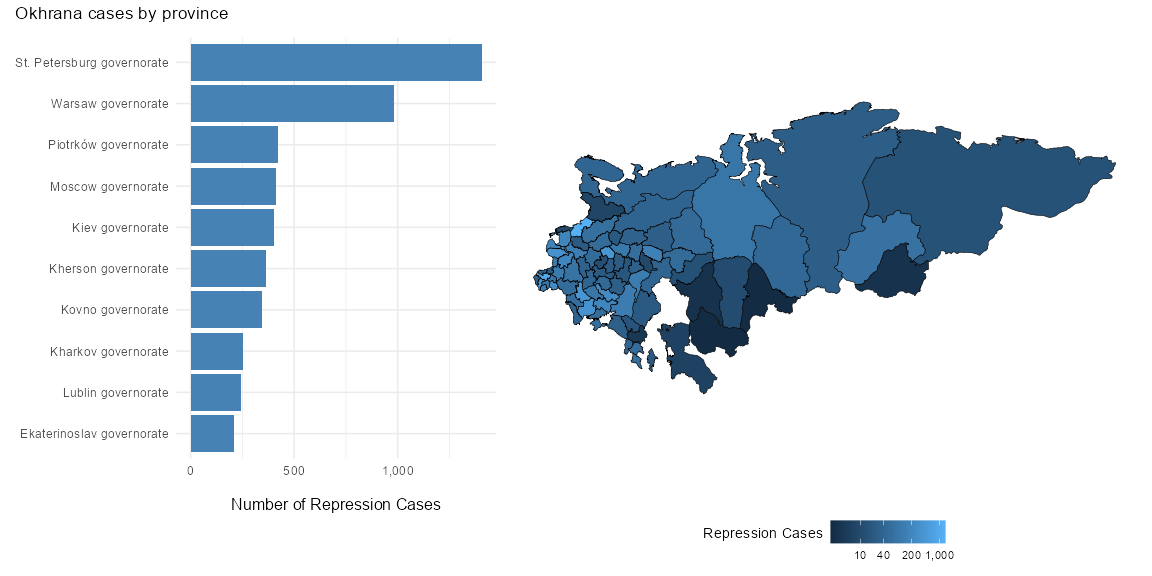
\includegraphics[width = \textwidth]{okhrana_by_province.png}
\end{figure}

Urbanization, by contrast, shows a strong and statistically significant association with surveillance levels in Models 4 and 5. This supports the view that urban centers—where ideologically framed opposition and labor agitation were more visible—were key targets for Okhrana activity. The marginal significance of the urbanization–inequality interaction term in Model 5 hints at a potential complementarity: repression was less intense where peasant land inequality coincided with urban density, though this estimate is imprecise. I plot it in \ref{fig:visualizing_urbanization_x_land_gini_interaction}. The negative sign on the interaction term suggests a possible substitution effect: in highly urbanized provinces, inequality may have been less politically salient as Marxist and labor-oriented ideologies supplanted land-based grievances. Still, due to imprecision and outlier sensitivity (notably Moscow and St. Petersburg), this result should be interpreted cautiously.

In sum, the results lend very limited support to a selective repression framework, where surveillance was responsive not merely to structural deprivation, but to its politicization through unrest and its proximity to centers of social agitation.

\section{Robustness checks}

\begin{table}
\centering
\caption{Robustness models specifications}
\label{tab:rob_model_specifications}
\resizebox{\ifdim\width>\linewidth\linewidth\else\width\fi}{!}{
\begin{tabular}[t]{lcccc}
\toprule
  & Control for population & Revolutionaries only & Alternative inequality measure & Negative Binomial\\
\midrule
Intercept & \num{-9.718}* & \num{2.241} & \num{1.208} & \num{31.326}*\\
 & (\num{3.881}) & (\num{1.557}) & (\num{1.076}) & (\num{43.501})\\
(Log) Pre-1905 unrest & \num{0.154} & \num{0.661}* & \num{0.465}+ & \num{1.799}*\\
 & (\num{0.265}) & (\num{0.262}) & (\num{0.260}) & (\num{0.420})\\
Land inequality (Gini) & \num{-1.877} & \num{-2.277} &  & \num{0.082}+\\
 & (\num{1.379}) & (\num{1.502}) &  & (\num{0.109})\\
Share of serfs (1858) & \num{0.302} & \num{-0.289} & \num{0.110} & \num{1.012}\\
 & (\num{0.619}) & (\num{0.670}) & (\num{0.686}) & (\num{0.604})\\
Peasant land share & \num{0.501} & \num{-0.601} & \num{0.553} & \num{0.475}\\
 & (\num{1.017}) & (\num{1.084}) & (\num{0.794}) & (\num{0.459})\\
Urbanization (1904) & \num{5.653}** & \num{4.182}* & \num{6.286}** & \num{593.362}***\\
 & (\num{1.644}) & (\num{1.782}) & (\num{1.827}) & (\num{934.820})\\
Manufacturing share (1904) & \num{1.221} & \num{2.336} & \num{0.216} & \num{0.709}\\
 & (\num{3.411}) & (\num{3.712}) & (\num{3.802}) & (\num{2.331})\\
\midrule
Num.Obs. & \num{48} & \num{48} & \num{48} & \num{48}\\
R2 & \num{0.577} & \num{0.390} & \num{0.445} & \\
R2 Adj. & \num{0.503} & \num{0.301} & \num{0.378} & \\
AIC & \num{520.2} & \num{472.8} & \num{529.4} & \num{531.2}\\
BIC & \num{537.1} & \num{487.8} & \num{542.4} & \num{546.2}\\
Log.Lik. & \num{-51.947} & \num{-56.729} & \num{-58.502} & \num{-257.593}\\
F & \num{7.806} & \num{4.377} & \num{6.725} & \num{7.637}\\
RMSE & \num{0.71} & \num{0.79} & \num{0.82} & \num{183.58}\\
\bottomrule
\multicolumn{5}{l}{\rule{0pt}{1em}+ p $<$ 0.1, * p $<$ 0.05, ** p $<$ 0.01, *** p $<$ 0.001}\\
\end{tabular}}
\end{table}

Table \ref{tab:rob_model_specifications} presents a series of robustness checks to validate the main findings. These include (i) controlling for provincial population size, (ii) using only Okhrana cases identified as “revolutionaries,” (iii) substituting an alternative measure of inequality, and (iv) re-estimating the model using a negative binomial specification to address count-data overdispersion. Negative binomial model's coefficients are expontiated to arrive at incident rate ratios. 

The positive relationship between pre-1905 unrest and Okhrana repression remains substantively similar across all models and reaches statistical significance in all cases but the i) model. This reinforces the interpretation that past mobilization—rather than latent structural features alone—was a central determinant of surveillance intensity.

The population-controlled model yields a reduced, though still positive, unrest coefficient, suggesting that part of the association may reflect broader demographic correlates of unrest. One could argue this is an artifact of the Russian Emprire demographics. Indeed, since most of the population were peasants, controlling for population size might obscure the effects of unrest, especially if more populous provinces received more land inequality. This is at least partly true because serfdom as an institution of labour coersion generally appeared because of labour, not land scarcity - and was used to tie peasants down in places where most labour was needed. 

Using only “revolutionary” cases as the dependent variable produces a slightly stronger unrest coefficient, further indicating that state targeting may have blended ideological and geographic cues - responding both to political content and to the spatial imprint of historical dissent.

The alternative inequality measure produces results in line with baseline models, reaffirming the null effect of inequality per se. Similarly, the negative binomial model confirms the main results under an alternative distributional assumption, with unrest remaining a statistically significant predictor.

Overall, these robustness checks do not do much to either reinforce or disprove thecore finding: that early rural unrest may have left a weak spatial legacy of suspicion and repression in the Tsarist surveillance regime, especially when filtered through the lens of urban transformation and ideological radicalization.

\section{Conclusion}

This paper shows that Tsarist repression, particularly that of the Okhrana, was neither indiscriminate nor purely reactive. Instead, it was spatially patterned: provinces with histories of peasant unrest faced more intensive surveillance, even decades after the initial disturbances. The data suggest that the Empire’s coercive apparatus treated prior mobilization as a proxy for future threat, especially when such unrest intersected with urbanization and ideological activism, which were traditional targets for the Imperial secret police.

Notably, structural variables like land inequality or serfdom alone did not predict repression; only where they had translated into contentious action did they elicit sustained state attention. This finding aligns with broader political economy models where elites repress rather than incorporate when inclusion would threaten their position.

Viewed through the lens of democratization, the Russian Empire’s trajectory is best understood as a blocked path. Reforms were partial and strategically designed to protect the social hierarchy. Zemstvos and the State Duma functioned less as a channel for peasant empowerment than as a constrained arena shaped by estate politics. In this context, repression was not just a response to unrest but a barrier to the emergence of a genuine participatory order.

% Bibliography
\printbibliography

\section{Appendix}

\subsection{Constructing land inequality Gini measure}\label{sub:constructing_land_inequality_gini_measure}

To quantify the distribution of landownership within provinces, I construct a Gini coefficient using bracket-level data on privately held land from the 1905 Statistika zemlevladeniya, digitized by Nafziger and Lindert. The source reports, for each province, the number of landowners and the total land area held within discrete holding brackets (e.g., 10–20 desiatins, 500–1000 desiatins), disaggregated by legal estate.

I begin by removing the composite category peasants (including obschestvas and collectives), since landholdings are already reported separately for peasants (private) and peasants (only obschestvas and collectives). The data are reshaped into a panel of province–estate–bracket observations. Each size bracket is assigned a midpoint to approximate average holdings; for open-ended intervals, I use 5 desiatins for holdings below 10, and 12,500 desiatins for holdings above 10,000.

The Gini coefficient is calculated within each province based on the cumulative distribution of owners and land across all legal estates. Letting $X_i$ denote the cumulative share of owners up to bracket $y_i$ and $Y_i$ the corresponding cumulative share of land, the Gini is computed as:

\begin{equation}
G = 1 - \sum_{i=1}^{n} (Y_i + Y_{i-1})(X_i - X_{i-1})
\end{equation}

This nonparametric formula corresponds to the area between the Lorenz curve and the line of equality. The resulting Gini coefficient provides a summary measure of land concentration within each province, incorporating variation both across and within formal legal estates. The magnitudes are in line with a similar calculation of \cite{lindert_russian_2014}. 

\end{document}